\chapter*{Conclusione} %Se si cambia il Titolo cambiare anche la riga successiva così che appia corretto nell'conclusione
\addcontentsline{toc}{chapter}{Conclusione} %Per far apparire Introduzione nell'indice (Il nome deve rispecchiare quello del chapter)
%
In conclusione, durante il mio tirocinio, ho sviluppato un'applicazione web basata su .NET MVC 6.0 con 
l'obiettivo di creare un servizio che automatizzasse in modo efficiente il 
processo di integrazione dei nuovi dipendenti, un passaggio cruciale e ricorrente per 
tutti i nuovi membri dell'organico aziendale.\ Questo progetto ha consentito 
all'azienda di mettere a disposizione uno strumento estremamente automatizzato, riducendo 
significativamente il carico di lavoro del dipartimento HR e delegando gran parte delle 
attività operative alla gestione automatizzata del sistema.
\\ \\ 
In particolare, il tempo di gestione del processo di Onboarding da parte del reparto HR  è il seguente:

\begin{figure}[H]
	\centering
	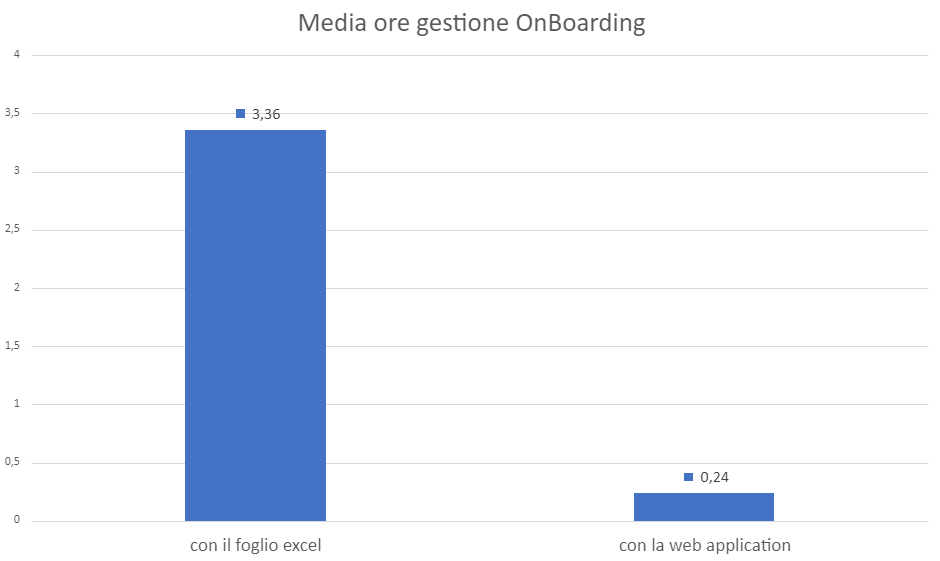
\includegraphics[width=\textwidth]{img/conclusione1.png}
	\label{fig:conclusione1}
	\caption[media ore di gestione del processo di OnBoarding]{\noteStyle{Nel grafico visualizzato, vengono considerati esclusivamente i periodi di tempo dedicati dal personale 
	del dipartimento HR alla coordinazione del processo Onboarding durante il suo ciclo per un utente specifico. I dati 
	temporali riportati sono calcolati come una media basata sui tre OnBoarding più recenti gestiti.
	È importante sottolineare che le informazioni fornite nel grafico non riflettono la durata complessiva del processo, 
	bensì rappresentano unicamente il tempo impiegato dal personale HR per garantirne una corretta gestione.}}
\end{figure}

Va notato che l'azienda, in virtù della sua certificazione ISO 9001, non solo è obbligata a farlo, 
ma si impegna attivamente a gestire e analizzare attentamente i feedback provenienti dagli utenti del sistema, 
con l'obiettivo di migliorarne costantemente l'efficacia e l'efficienza.
\\ \\
L'applicazione web, pur rispettando appieno tutti i requisiti aziendali iniziali, 
offre un ampio margine per ulteriori miglioramenti, come discusso dettagliatamente nel capitolo dedicato del documento~\ref{chapter:Risultati_e_sviluppi_futuri}, 
offrendo così opportunità significative per un futuro sviluppo e ottimizzazione.